\subsection{Ambient Light}

\begin{frame}{Ambient Light - Global Illumination Approximation}
  \begin{columns}
    \begin{column}{0.6\textwidth}
      \only<1-2>{
        \begin{conceptbox}{Direct Lighting Problem}
          \small
          Real scenes have indirect lighting
          \begin{itemize}
            \item Light bounces off walls, ceiling
            \item Reflections illuminate shadows
            \item Even "dark" areas receive some light
          \end{itemize}
        \end{conceptbox}
      }

      \only<3>{
        \begin{raybox}{Solution: Ambient Light}
          \small
          Add constant ambient term
          \begin{itemize}
            \item Prevents completely black shadows
            \item Approximates global illumination
            \item Simple and fast to compute
          \end{itemize}
        \end{raybox}
      }
      \only<4->{
        \begin{conceptbox}{Ambient Light Parameters}
          \textbf{Ambient intensity:} $\mathbf{I}_l$ (constant)
        \end{conceptbox}
      }
    \end{column}
    \begin{column}{0.4\textwidth}
      \only<1>{
        \begin{tikzpicture}[scale=0.8]
          \draw[thick] (0,0) -- (3,0) -- (3,3) -- (0,3) -- cycle;
          \node[circle, fill=LightColor, minimum size=0.6cm] (light) at (1.5,2.5) {};

          \draw[lightray] (light) -- (3,1.5);
          \draw[lightray] (light) -- (0,1.25);

          \draw[lightray, dashed, opacity=0.6] (3,1.5) -- (2,0);
          \draw[lightray, dashed, opacity=0.6] (2,0) -- (1,0.5);
          \draw[lightray, dashed, opacity=0.6] (0,1.25) -- (0.5,0);
          \draw[lightray, dashed, opacity=0.6] (1,0.5) -- (0.75,0);

          \node[sphere, minimum size=0.6cm] (obj) at (1,1) {};

          \node[right] at (3.2,2) {\footnotesize Direct light};
          \node[right] at (3.2,1) {\footnotesize Bounced light};

          \node[below] at (0.625, 0) {\footnotesize Indirect light};
        \end{tikzpicture}
      }
      \only<2->{
        \begin{figure}
          \centering
          \only<2>{
            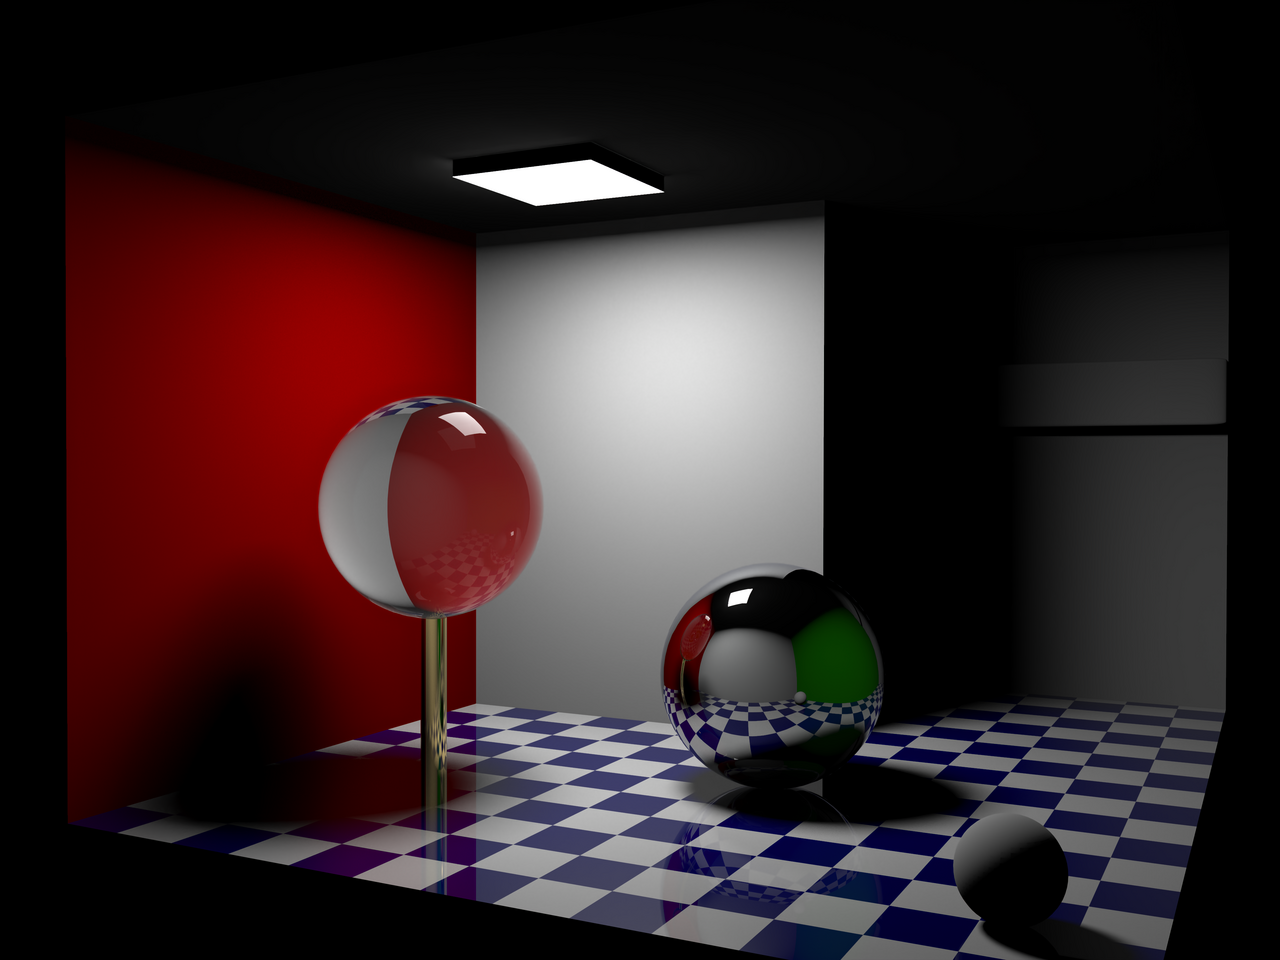
\includegraphics[width=0.8\textwidth]{images/no_gi.png}
            \caption*{Only direct light}
            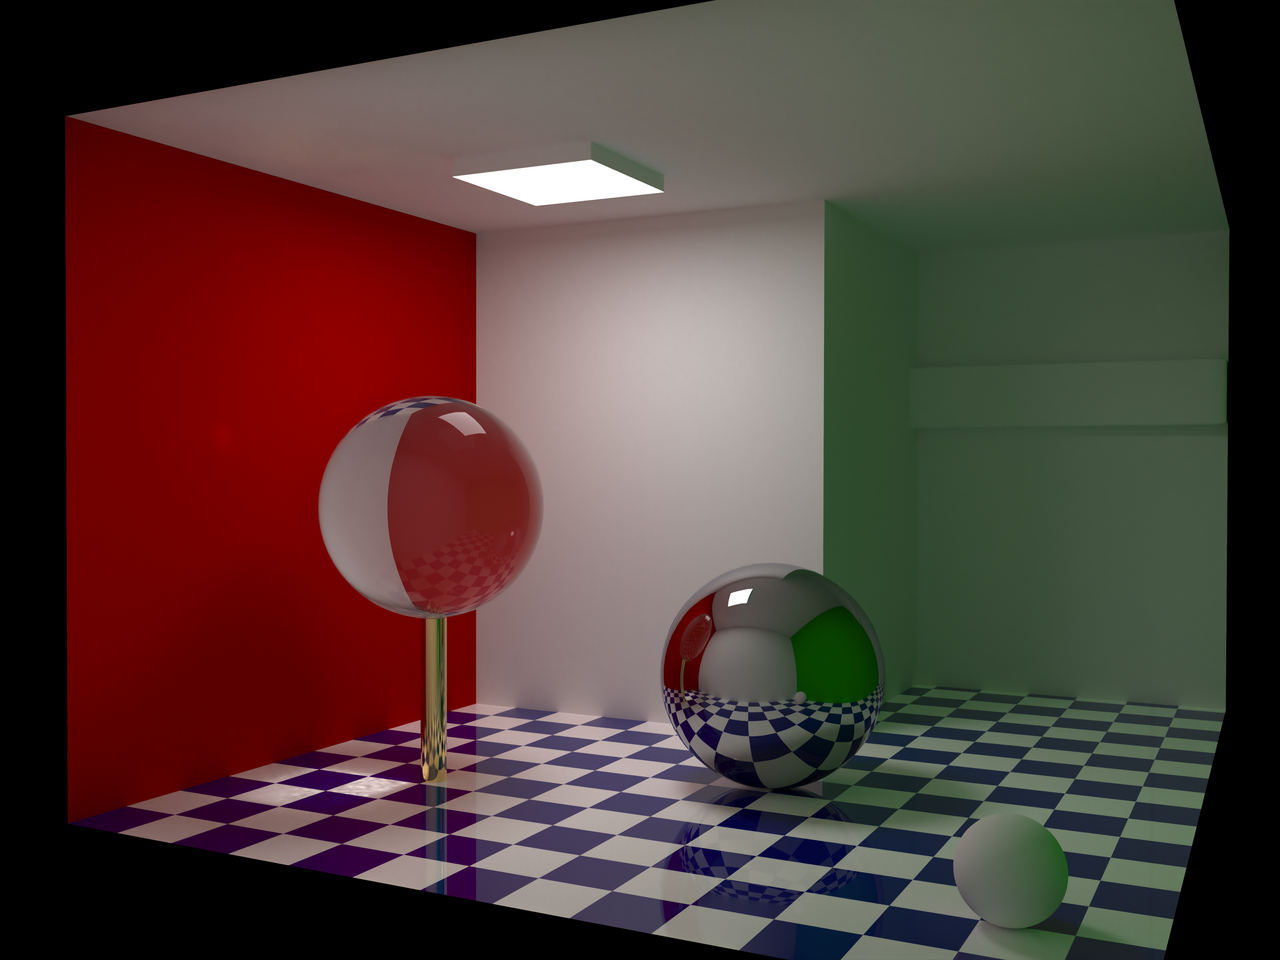
\includegraphics[width=0.8\textwidth]{images/gi.png}
            \caption*{Global illumination}
          }
          \only<3->{
            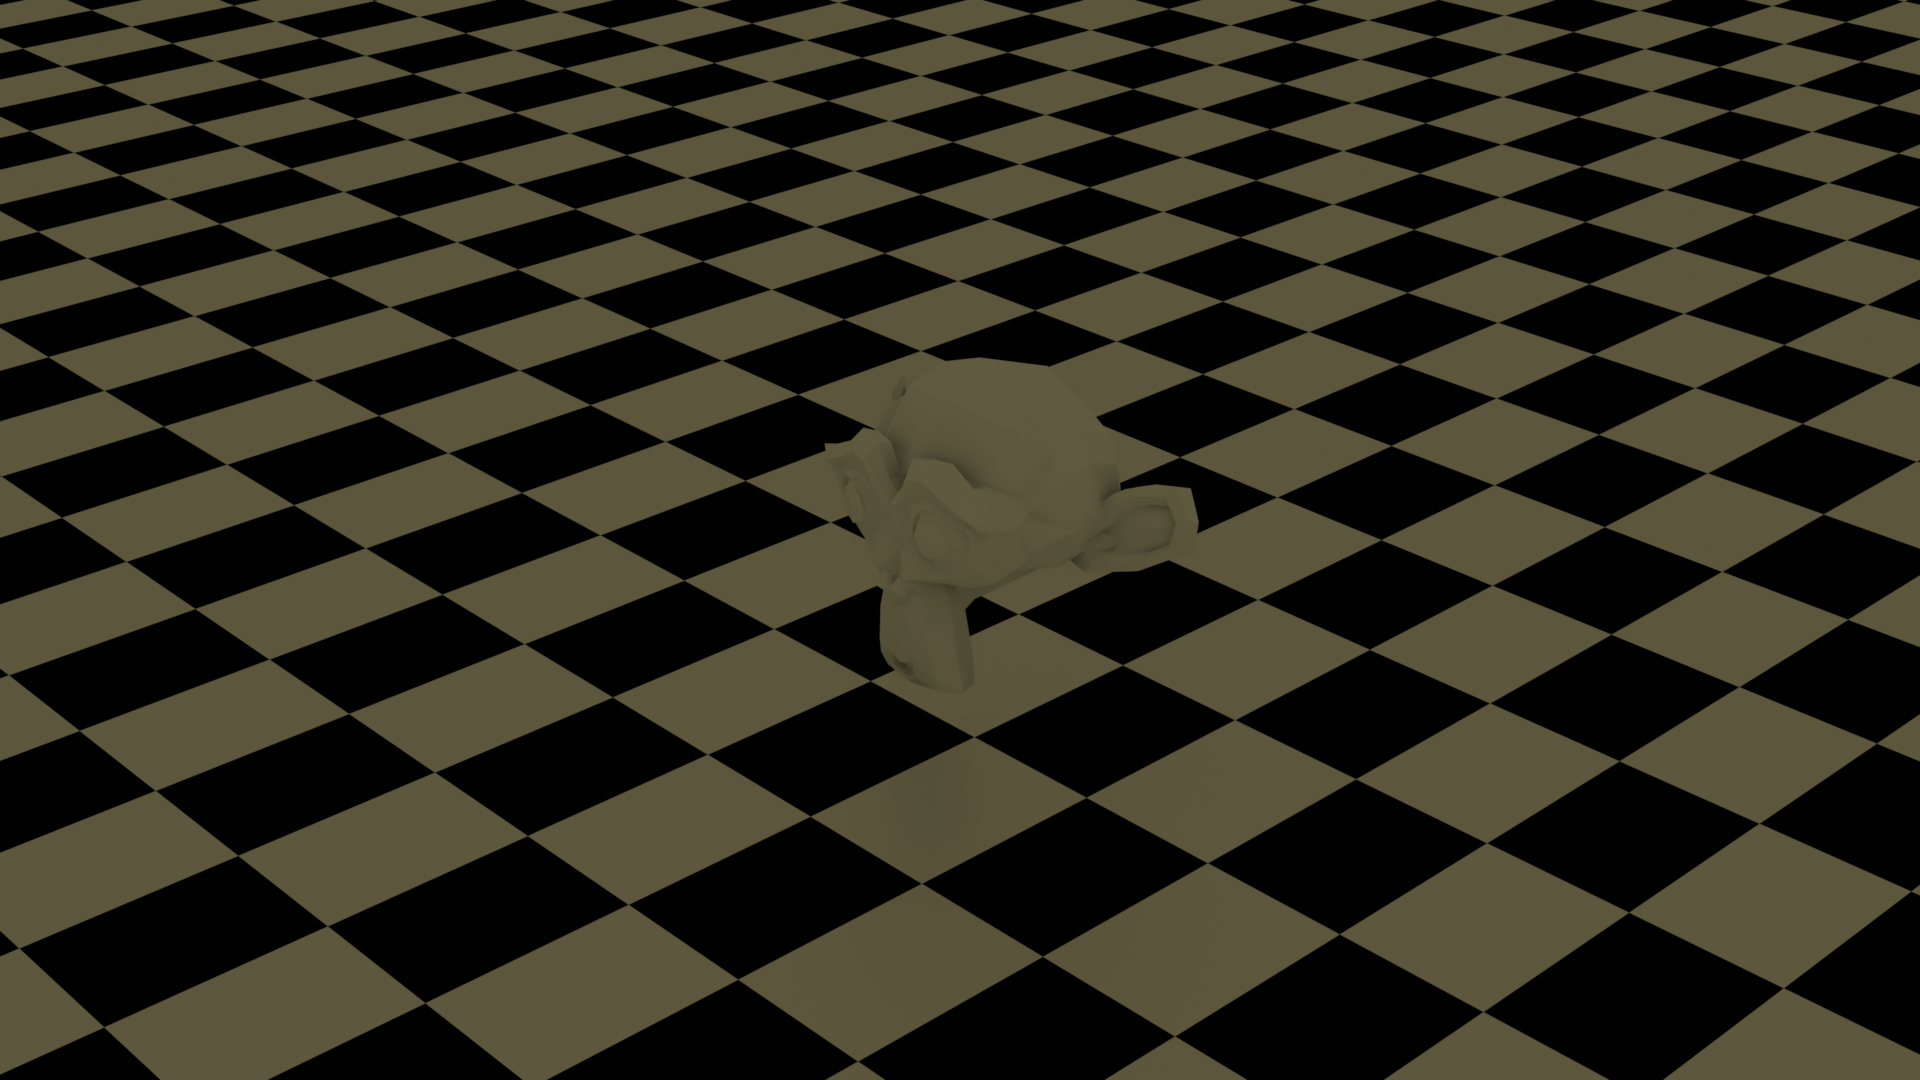
\includegraphics[width=0.8\textwidth]{images/ambient.png}
            \caption*{Ambient light ft. Suzanne the monkey}
          }
        \end{figure}
      }
    \end{column}
  \end{columns}
\end{frame}
